\chapter*{Introduction}
\label{ch:Introduction}
Lyrics serve as one of the main foundations of songs, playing a crucial role in
expressing feelings in many different ways.
The emotional tone of songs can serve various purposes, such as
automatized playlist creation or songs' organization,
offering an alternative to the more traditional genre-based classification. \\
%Analyzing the emotional tone of song texts can give useful insights about individual mental states, cultural trends, social issues and more.
% The main goal of this project is to perform emotion detection on stanzas of songs.
% The goal of this project is the development of 4 Machine Learning models
% that perform emotion detection on songs' stanzas.
To obtain a deeper understanding of emotional fluctuations within the texts,
the models assign emotion labels to individual stanzas instead of full songs.
The emotion labels correspond to Robert Plutchik's eight primary emotions
(shown in figure~\ref{fig:primary_emotions}), providing a comprehensive range
for representing various emotional states.\\
\begin{figure}[H]
    \centering
    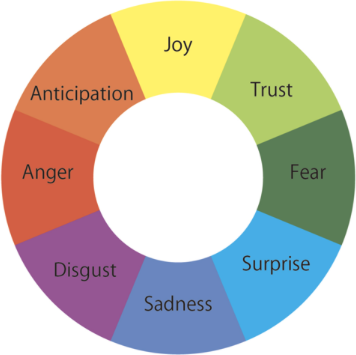
\includegraphics[scale= 0.25]{pictures/plutchik_primary_emotions.png}
    \caption{Plutchik's eight primary emotions}
    \label{fig:primary_emotions}
\end{figure}

This report aims to clearly cover and illustrate various aspects of the work. 
The \textit{Methods} chapter contains a detailed explanation of the data and
procedures used in the project, providing descriptions of each part implemented
in the project.
The \textit{Results} chapter presents an overview of the
obtained outcomes.
These results are further explored in the final sections, \textit{Discussion}
and \textit{Conclusions}, which interpret the general findings, recap the
primary objectives of the work, and discuss the importance or potential
applications of the results.